\documentclass[12pt]{scrartcl}
\usepackage {ucs}
\usepackage{graphicx}
\usepackage[utf8x]{inputenc}
\usepackage[T1]{fontenc}
\usepackage[ngerman]{babel}
\usepackage{hyperref}
\usepackage{nameref}
\usepackage{amsmath}
\usepackage{amssymb}
\usepackage{array}

\begin{document}

\title {Documentation}
\section {OCRe - Optical Character Recognition - experiment}
This is a naive approach to optical character recognition, as one of the most important aspects in its creation was simplicity. OCR is a widely used from reading road signs on mobile phones for translation, scanning of documents - for the sake of digitalization and the ease of use with a computer, to automatically translate manuscripts of old languages in order to decypher them, or to make handwriting machine-readable. Therefore there are many projects out there that are highly complex and use multiple techniques of character recognition to improve on their quality.

Nowadays many OCR-engines rely on neural networks, that deliver quite a good performance but need appropriate training beforehand. It is also sometimes needed to dive into the context of the text in order to clarify ambiguous possibilities. However, OCR cannot be done to 100\% accuracy as we will see later. Also I did not implement context or semantic word checking as it would have clearly gone beyond a university project to be done singlehandedly within half a semester.\newline
The most known engine is certainly the Tesseract engine that is owned and was open sourced by Google.\newline
There exist many other engines that are written in Python and use Keras/TensorFlow for neural networks. Many of them are abandoned projects, though.


\subsection{choices made}
OCR can be separated into 3 main branches for similarity measures used.
\begin{itemize}
\item Feature matching
\item pattern matching
\item neural network (a mixture of both depending on the engine and the task)
\end{itemize}

For ease of implementation reasons this project uses \textbf{pattern matching}.\newline
Feature extraction like finding common lines, such as 'A' consisting in its idea of 3 crossing lines but an '8' of 2 circles, not mentioning 'g' in its various forms and '"' being in its core twice the character ' for instance, would not be feasible to implement in such a short amount of time.

Layout detection and image improvements (rotation, smoothing, ...) would be a nice-to-have, but were not the focus of this project.

I was concerned how to find the actual letters without pushing a window withrough the lines that could potentially contain more than one character - for the case that some small letter would be overshadowed by W or T. (like iT, or iW combinations). To counteract this and enable pattern matching for different sized input and training letters deblobbing and rescaling to a mask was chosen.
Unfortunately it resulted in loss of ratio. Therefore I l . | - \_ all have the same mask: a completely black square. Also x and X and c and C would be hard to distinguish.\newline

The masks' size was chosen to not change the ratio too much for most letters and deliver decently recognizable images. 

A more sophisticated training image generation pattern, or deliverance of line information and position could help, but may end up in a lot of switch cases, and thus generate a lot more work. For this kind of project, recognizing most of the letters was good enough, as the focus was on the modelling and C++ and not so much, if the program is ready for general use.

For loading of images and filesystem operations (iterating through the training-image folder) the boost GIL and filesystem library (ver. 1.68) was used.


\section {System Model}
  \subsection{System Diagram}
\begin{figure}[h]
\centering
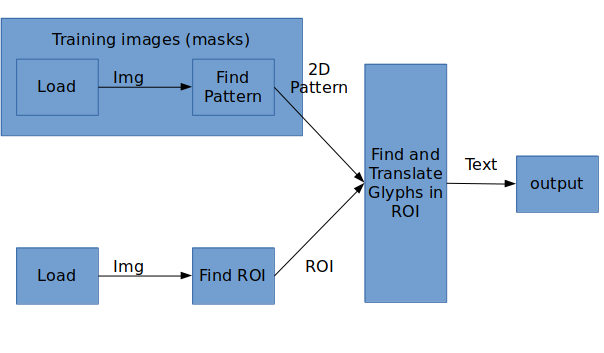
\includegraphics[width=\textwidth,keepaspectratio]{./systemdiagramm.png}
\end{figure}
\newpage

  \subsection{Concepts}
\begin{itemize}
\item Image: The image to be read. JPEG (i.e. '.jpg') is the only image format supported up to this point.\newline
\begin{tabular}{ m{6cm} m{7cm} }
\hline
read\_image([path]) -> matrix & loads image from disk and copies the image's contents into a newly created matrix.\\
\hline
\end{tabular}
\vspace{1cm}


\item Matrix: A matrix is a 2 dimensional image representation. For ease of use I used (std::)vectors of vectors of integers. Up until the binarization, that happens in gly\_scan(), most matrices could potentially be replaced by (sub)views of the actual image loaded to reduce copying. (some work provided)\newline
\begin{tabular}{ m{6cm} m{7cm} }
\hline
to char(matrix, translation\_table) -> matrix & compares the matrix with the masks in the translation matrix to find the best fit\\
\hline
matrix(matrix input, height, width) -> matrix & creates new matrix and stretches or compresses the areas\\ 
\hline
matrix(Set)-> matrix & creates a matrix from a set of points\\
\hline
\end{tabular} 
\vspace{1cm}

\item Masks: Masks are binarized matrices of fixed size, that are ready to be compared to one another.\newline
all expressions that are valid for matrices, are valid for masks
\vspace{1cm}


\item Lines: 2 dimensional subsets of the initial image. Again they could potentially be replaced by subviews in a later version.\newline
all expressions that are valid for matrices are, valid for lines
\vspace{1cm}


\item Glyph: The class glyph contains a set of pixels, that are darker than a certain threshault $T*255$. They are obtained by gly\_scan([line]). Upon discovering a new pixel the constructor issues the method findall(), that finds all directly connected pixels. This is an assumption, that may or may not be useful depending on the character set and the quality of the scan.\newline
Glyphs can be compared for equality, such that if any pixel is found in an existing glyph those 2 glyphs must be identical. Which is the logical conclusion of the before mentioned assumption.\newline
For some characters like i or j (or ; or : respectively) glyphs must be fused, which poses another threat to the accuracy or in this case disambiguity as will be seen later on.\newline
\begin{tabular}{ m{6cm} m{7cm} }
\hline
glyph1==glyph2 -> bool & checks for equality. returns true, if one pixel of one glyph is contained in the other\\
\hline
glyph1.fuse(glyph2) -> void & fuses glyph 2 with glyph1\\ 
\hline
glyph.contains(point) -> bool & returns true, if pixel is contained in the glyph\\
\hline
\end{tabular}
\vspace{1cm}


\item Translation Table: A translation table is the key to translate masks of glyphs into corresponding characters. It is being made in the thread 1 while the main thread issues the scanning of lines for glyphs.\newline
only needed by to\_char() as an argument. is is being created by make\_masks();
\vspace{1cm}

\item similarity measure: To compare 2 masks an abstract distance measure is being needed. In the basic form, every pixel that is not the same for the input and the mask to be tested against, gets a penalty point. The mask that has fewest points for the input mask is most likely to be the correct character.\newline
\begin{tabular}{ m{6cm} m{7cm} }
\hline
similarity(matrix1, matrix2) -> score(double) & compares 2 matrices for similarity. Matrix 1 and matrix 2 must have the same dimensions\\
\hline
\end{tabular}
\vspace{1cm}

More advanced approaches pay a heavy toll on timely performance, as we will see later, as every pixel may go through several iterations of checks to find a more informative score.\newline

\end{itemize}

  \subsection{workflow}
In this project the following steps are being issued as follows:\newline
Thread 0
\begin{itemize}
\item thread 0
  \begin{itemize}
    \item issue thread 1 to simultaneously create masks
  \end {itemize}
\item thread 0 then looks to reduce the window to be scanned to a minimum and finds separate lines
\item these lines are then one-by-one (or in parallel) provided to the recognition subsystem, which:
  \begin{itemize}
  \item scans the line for glyphs (gly\_scan) and fuses composed glyphs
  \item due to the order of scanning the characters need to be sorted by their x-coordinate  
  \item transforms the glyphs to a matrix, resizes to a mask and then tests for similarity against the provided masks of the set of characters in the folder 'Trainingimages' to find the corrseponding ASCII char  
  \item then empty spaces are to be inserted into the almost ready string
  \item which will then be the outcome of the procedure
  \end{itemize}
\item these strings that were produced by each line are then concatenated to form the final multi-line string
\end{itemize}

\section {Performance: Accuracy vs Speed}

In this section the aforementioned issues and assumptions will be discussed.

\subsection {accuracy}
The accuracy is highly dependent on what parameters are provided to the char recognition process.

Recognition can fail on multiple occasions: Be it in finding lines (for instance by overlapping or outliers), finding glyphs, correctly fusing composite glyphs or finding the correct corresponding char for each glyph.

As mentioned before in section above, the choices and assumptions made are having a huge impact on recognition quality: Such as loss of ratio and therefore ambiguity for certain characters. The similarity measure is the other obvious place for improvement. However it may come with a cost.

Due to image compression and scanning properties pixels may be scarce and therefore not connect to a single glyph or completely be misplaced as outliers. Here lie some one of the biggest issues. 

If the threshault T is too big (resulting in only white being recognized as white) there could be cases where some characters that should be separate are scanned into a single glyph and therefore recognition will fail.\newline
Such a case can even happen for 100\% quality jpegs when characters are being pushed closer together due to some rules for a font, as in this example for 'fi' that is then translated into 'h' or 'n'. So unfortunately the one-glyph-one-char assumption was not correct but still holds the basis for a rather simple model and can be used for some cases.

If on the other hand T is being made too small and only values close to 0 are being regarded as black, the assumption will see another fail as some single pixels that keep the glyph together may drop out and fragment the char into different glyphs and therefore also resulting in a failing character recognition.

These issues may be fixed by some algorithms that tend to tendencies and gradients. For instance by artificially creating subpixels and increasing the sampling rate (pixels per length) allowing for a smoother transition from one glyph to the next and also going from maximal black to maximal white and back again and creating the wanted separation. However it can result in more computation to be necessary and copying of data.

An enhancement could be further provided by redefining black and white and therefore increasing the contrast.

All in all larger letters (with enough space between one another) certainly will benefit the task of character recognition as well as better picture quality (pixels per length).

Factors that can further influence accuracy are extra pixels created by rotation, de-trangularization and rescaling of parts of the image. Those matters will not be further discussed here.

Picture quality aside, one of the most important parts, though, is font. Be it handwritten, old fashioned, with or sans serif, italic fonts vs non italic fonts.

Whoever tried to decypher someone else's handwriting knows that OCR cannot be done to 100\% accuracy even by humans. Ironically the simpler sans serif fonts, for our simple case of machine written text, pose a larger threat, as they are mostly reduced to the main features of the respective letters. Such that I and l are only distinguishible by the context. Is the context unknown, there is no chance to know what the result is meant to be. Contexts such as abbreviations can be particularly bad: as 'lol', that stands for 'laughing out loud', could be turned into 'IoT' (Internet of Things) with a single crossbar over the second vertical line representing the 'l', and thus the first 'l' turns into an 'I'. Now these are common abbreveations these days, but turn to a topic completely unknown and intuition will be lost.


\subsection {speed}
It certainly is useful to fit the boundaries tight to minimize the overall calculations, where nothing is to be expected.

Also binarization at an early stage can provide a speedup due to needing only 1 bit per pixel (at the potential cost of the aforementioned accuracy loss) compared to 4bytes for each integer.

The model has various places for parallelization, be it multithreading or SIMD instructions. Most of the uses for std::transform() are parallelizable. Those that are not are commented in the code for race condition issues. So by making the writeing or accumulating operation atomic it would also be parallelizable. The easiest example therefore is the recognition of single lines, that can happen in parallel.

Larger images with more pixels will benefit the accuracy but also increase the number of computations required.

Probably the most impacting factor in speed is the choice of similarity measure. This project has 2 possibilities implemented. One plain and clear: "if the same pixel for both comparing masks is different, there is going to be a penalty". And the other is a distance measure: "how far is the next same colored pixel?"

The first one is highly parallelizable as every pixel is independent from one another, and needs to be visited only once. The second variant yields slightly better outcomes but is also a lot slower as the complexity goes from O(N) - with N being the number of pixels in a mask - to O($N^3$). Even though not all pixels have to be repeatedly visited the second variant has a lot of if-clauses resulting in branching and therefore pipeline stalls and also possibly a lot of memory transactions.

It may prove to be interesting if some sort of 2 dimensional dynamic time warping algorithm was implemented to find the best fit for slightly offset masks aswell as provide a precise measure of how far off the image is. The variance over all the pixels could eradicate an offset and put more emphasis on the total structure of the pattern and the features and less on the relatively random occurrence of pixels. However the normal DTW algorithm for a 1 dimensional series is already O($N^2$). If such an algorithm exists, it will hardly be better than O($N^4$) which will have to be bought with considerably smaller masks. However losing the information on position and ratio should provide a good enough approach with the second approach as the masks are already aligned, if the character is the correct one.

\section {Why C++?}
C++ has the benefit of having widespread use, well tested and optimised libraries and compilers that are well optimized, that can eat a lot of work at compilation time and really occupy a CPU's core. Its abstract template system can generalize a function for other data types and its type system is strict to halt compilation to give beneficial feedback to the developer giving exact control instead of just letting minor irregularities pass by. In this case most of the parameters were only known at runtime, so that not many things can be modelled generally and folded and squared away by the compiler. Modern features like type deduction, operator overloading and the aforementioned template functions can make clean and overall precise, understandible and expressive code.
C++ allows to use a formal style and its deterministic memory management will allow for complete control over what is happening when. 



\end{document}

